\documentclass{article}


\title{Hashing and Bloom filters key lookup comparison}
\author{names}
\date{\today}


\usepackage[backend=bibtex]{biblatex}
\usepackage{graphicx}
\usepackage{amsmath}
\usepackage[a4paper, total={5in, 8in}]{geometry}


\bibliography{references}
\nocite{*}

\begin{document}
    \maketitle
    \thispagestyle{empty}
    \begin{abstract}
	This is the abstract of the document is the abstract of the document is the abstract of the document is the abstract of the document is the abstract of the document
	is the abstract of the document is the abstract of the document is the abstract of the document is the abstract of the document is the abstract of the document
	 is the abstract of the documentis the abstract of the document is the abstract of the document is the abstract of the document is the abstract of the document
	 is the abstract of the document  is the abstract of the document is the abstract of the document is the abstract of the document is the abstract of the document
	 is the abstract of the document is the abstract of the document is the abstract of the document is the abstract of the documentis the abstract of the document
    \end{abstract}
	

    \section{Introduction}
        This project is mainly aimed at learning different implementations of hashing based data structures and their effectiveness in applying a dictionary search problem. \\\\
A dictionary is used to maintain a set under insertion and deletion of elements while membership queries provide access to the data. The most efficient dictionaries, in theory, and practice, are based on hashing techniques. \\\\
To achieve different results and build a complete analysis, we have proposed searching with two types of dictionary data structures: hash tables and bloom filters. \\\\
The main performance parameters that we are going to study, analyze and contrast along this research work are: lookup time, build time, average probes and false positives.
All the algorithms have been implemented in c++ and the same data has been applied to the execution of different versions of the same experiment. 

    \section{Experiment pipeline and methodology}
    	The experimentation process was a very tedious task since it required to take in account a lot of parameters. TODO(Add pipeline image)
    	\subsection{Open Addressing}
Open addressing is one of the two main methods of collision resolution in hash tables. The four main techniques are:

\begin{itemize}
    \item \textbf{Linear probing:} its principle is accomplished using two values: a start index and a stepping value. When a collusion occurs, the table is search sequentially for an empty slot adding repeatedly the second value to the first until either a free space is found or the entire table is traversed.
    \item \textbf{Quadratic probing:} its principle is accomplished using four values: a start index, a stepping value and two constant values. When a collusion occurs, an arbitrary quadratic polynomial value -made by the combination of all the values but the start index- is added to the first one; the finish criteria is the same as the previous technique. The idea is to skip regions in the table with possible clusters.
    \item \textbf{Double hashing:} its principle is accomplished using two values: a start index, a stepping value and a third value. When a collusion occurs, the combination of the stepping and the third value is added to the first one; the finish criteria is the same as the first technique. The idea is to tackle effectively clustering problems.
    \item \textbf{Cuckoo hashing:} its principle is accomplished using two values and either position is computed by the first or the second. When a collusion occurs, the key in the position is replaced and the replaced key is assigned to the position given by the other value. If this new position is occupied, the procedure is repeated until the key is inserted or the iteration reaches an arbitrary value. The replacement behaviour may result in an infinite loop. 
\end{itemize}
\begin{center}
\begin{tabular}{c|c}
    Technique & Function\\
\hline
    LP & h(k,i) = (h(k) + i) mod $m$ \\
\hline
    QP & h(k,i) = (h(k) + $c_1$i + $c_2i^2$) mod $m$ \\
\hline
    DH & h(k,i) = ($h_1$(k) + i*$h_2$(k)) mod $m$ \\
\hline
    QH & h(k) = $h_1$(k) or $h_2$(k) \\
\end{tabular}

\begin{tabular}{c|c}
    Parameters & Meaning \\
\hline
    k & key, value to insert or to search \\
\hline
    i & stepping value \\
\hline
    $c_1$, $c_2$ & constant values \\
\hline
    h(),$h_1$(),$h_2$() & hash functions \\
\end{tabular}
\end{center}

    \subsection{Separate Chaining}
    
    \subsection{Bloom filters}

    \section{Data Generation}
        The data used in each of the experiments consisted of a sequence of unsigned integers,  
        the data was written in two different files. One file contained the keys to insert into the dictionary and the other the text to find in the dictionary. 
       
		\subsection*{Linear Congruential Method}
		The randomness of the keys was based on the Linear congruential method (LCM) \cite{BOOK:2}. 
		We needed to have experiments as reliable as possible thus we needed a way to control the data generation, 
		that is why we used this method. The LCM is one of the oldest and best-known random number generators, 
		it is also very easy to implement. This method generates a cyclic sequence of numbers based on an initial seed. 
		Given a seed $X_0$ it is possible to generate the next number in the sequence 
		\begin{equation}
		X_i = (X_{i-1} * a + c) \, \bmod m
		\end{equation}
		 where $a$ is called the multiplier, $c$ the incrementer and $m$ the modulus. 
		 The size of the sequence depends on the parameters used, independently on the initial seed.
		  We used a combination of parameters that yield the maximum size sequence, that is parameters that yield $m$ numbers.  
		  This ensured us that that there where never repeated numbers in either of the two files since the size of $m$ was
		  sufficiently big. 
		  
		   
    \section{Experiment parameters}
    An experiment is purely defined by the subject, represented by the dictionary to test, and the parameters in each the dictionary was specified and tested. 
    \begin{itemize}
    \item \textbf{Size of $n$:}
		   The keys file contained n numbers and the text contained $2 * n + p * n$ where $p$ is the percentage of keys that are already inserted in the dictionary. 
		   We had a lot of discussion in which $n$ used and we tried different combinations but they yielded very similar results so we finally chosed an $n=10e^7$. 
		   That happens to be 10 million keys that where inserted into the dictionary, although the table size was much bigger. We tried to used a bigger size of $n$
		   but we encountered the size of the files we created where extraordinary big, we tried to divide the files but that wasn't of much use since we stilled needed to 
		   save all the numbers in the hash tables. When we tried to to this the linux oom-killer killed to process because of the out of memory that was caused. Nevertheless 
		   other researches \cite{ARTICLE:2} used similar sizes of $n$ so this size wasn't really an issue. 
    \item \textbf{Number of repetitions $Q$:}
    		   Each experiment was defined by a series of parameters to get the best results and avoid overfitting of the data to a single sample we 
    		   repeated each experiment with $Q=100$ that is we performed the same experiment $100$ times and averaged the results. 
   
   \item \textbf{Load factor $\alpha$:}
   		   The load factor is one of the variables that really helps into comparing each type of dictionary implementation, we used in total 
   		   $9$ different load factors ranging from $0.10$ to $0.9$ with an offset of $0.10$. We could have subdivided the interval with a lower 
   		   offset but after experimenting we found that there wasn't really a substantial difference. 
   		   
   \item \textbf{Key percentage $p$:}
   		  The key percentage represents the percentage of keys that are in the keys (inserted in the dictionary) that are in the search file (the second file where the lookups are done). 
   		  This variable did not have a big impact in the results since we average the lokuup time of each key individually and even if we chosed a really low key percentage we had a big enough 
   		  $Q$ that it didn't matter. Thus we chosed $p=0.5$;
   		  
    \item \textbf{Number of hash functions $k$:}
    		 This was a difficult parameter to choose since it had to be chosen optimally because if had a very big k then the number of false positives might diminish, but only if the size of the table
    		 was big enough, on the other hand if we chosed a small value of $k$ the table would fill more slowly but it was more probable to find to keys with the same bits mask. To decide into what to choose 
    		 we simply tested different values of $k$ with different results. 
    		 
    \item \textbf{Hash functions:}
    		The hash functions we chosed where not the purpose of this experiment altough we tried to choose. 
    		
    \item \textbf{Random seed:}
    		The seed number is really a determining factor into how the dictionaries will perform since different seeds yield to different keys and conscuently differnet hash outputs. 
    		That is why for each experiment we chosed the same initial seed, altough the next seed was chosen at random based on the initial seed, this enabled reprodudability. In total 
    		a number of $Q$ different seeds were selected, because the results of the $Q$ repetitions where average this enabled us to remove any outliers that could happend choosing a specific seed value. 
    \end{itemize}
    \section{Results}
    All the results that were obtained are specifically compared to the load factor of the table since it is a determining parameter in the efficiency of each dictionary. 
    
    	\subsection*{Speed performance}
    	To compare the speed...
    	\subsection*{Probes metric}
    	In this section we compare the average probes that were introduced in each search query...
    	\subsection*{False positives}
	    	This section is specifically centred in the false positive rate of the bloom filters...
	    	\begin{figure}[h!]
		  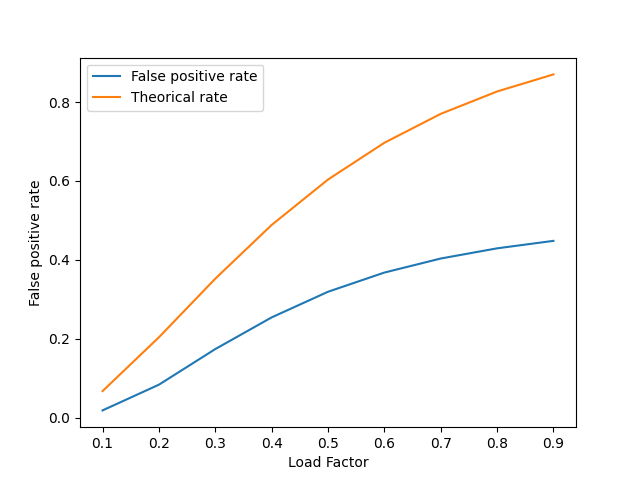
\includegraphics[width=\linewidth]{images/loadFactor_vs_falsePositives.png}
		  \caption{False positive rate comparison}
		  \label{fig:False positive rate}
		\end{figure}
    	
    	
    

    \section{Discussion}
	WE LEARNED THAT....


    \printbibliography

\end{document}
